\documentclass[12pt]{article}
\def\beqselinestretch{1.2}
%% packages called by Slava
\usepackage{xcolor}
\definecolor{darkblue}{rgb}{0.1,0.1,.7}
\usepackage[colorlinks, linkcolor=darkblue, citecolor=darkblue, urlcolor=darkblue, linktocpage,pagebackref]{hyperref} 
\usepackage[english]{babel}
\usepackage{amsmath,amssymb,graphicx,enumerate,bbm}
\usepackage{booktabs}
\usepackage{multirow}
\usepackage{geometry}
\geometry{letterpaper,tmargin=2.5cm,bmargin=2.5cm,lmargin=1.8cm,rmargin=1.8cm}
\usepackage[margin=10pt,font=small,labelfont=bf]{caption}
%\usepackage{mcite}
\usepackage{dsfont}
\usepackage{titlesec}
\titlespacing\section{0pt}{12pt plus 4pt minus 2pt}{0pt plus 2pt minus 2pt}
\titlespacing\subsection{0pt}{12pt plus 4pt minus 2pt}{0pt plus 2pt minus 2pt}
\titlespacing\subsubsection{0pt}{12pt plus 4pt minus 2pt}{0pt plus 2pt minus 2pt}
\titleformat*{\section}{\large\bfseries}
\titleformat*{\subsection}{\normalsize\bfseries}
\titleformat*{\subsubsection}{\normalsize\it}
\titleformat*{\paragraph}{\normalsize\bfseries}
\titleformat*{\subparagraph}{\normalsize\bfseries}
%\usepackage{cite}
\usepackage[noadjust]{cite}
\usepackage[utf8]{inputenc}
\setlength{\parindent}{0pt}
\setlength{\parskip}{0.5em}

\numberwithin{equation}{section}

%\usepackage[tocgraduated]{tocstyle}
%\usetocstyle{standard}

%\usepackage[titles]{tocloft}
\usepackage{tocloft}
\setlength{\cftbeforesecskip}{3pt}
%\setlength{\cftbeforechapskip}{3pt}
%\usepackage{chngcntr}
%\counterwithin{figure}{section}

\usepackage{etoolbox}
\apptocmd{\thebibliography}{\setlength{\itemsep}{0em}}{}{}

\begin{document}
	
	\vspace*{-.6in} \thispagestyle{empty}
	\begin{flushright}
	\end{flushright}
	
	\vspace{.2in} {\large
		\begin{center}
			%\resizebox{\textwidth}{!}{
			\bf  Possible superconductivity in $\pi$-flux Hubbard model
		\end{center}
	}
	\vspace{.2in}
	\begin{center}
		{\bf 
			Xiao-Yang Shen$^{1}$
		} 
		\\
		\vspace{.2in} 
		{\it $^{1}$Department of Physics, Tsinghua University, Beiing 100084, China}
	\end{center}

	\vspace{.2in}


\begin{abstract}
  
  
\end{abstract}
\vspace{.3in}
\hspace{0.7cm} 
%{\small \setlength{\parskip}{0pt} \tableofcontents}
\section{Introduction}
\section{$\pi$-flux Hubbard model}
The model describes the Hubbard model with $\pi$-flux,
\begin{equation}
	\hat{\mathcal{H}}=-\sum_{\langle\mathrm{i}, \mathrm{j}\rangle, \sigma}\left(t_{\mathrm{i}, \mathrm{j}} \hat{c}_{\mathrm{i} \sigma}^{\dagger} \hat{c}_{\mathrm{j} \sigma}+\mathrm{H.c.}\right)+ U\sum_{\mathbf{i}}\left(n_{\mathbf{i}\uparrow}-\frac{1}{2}\right)\left(n_{i\downarrow}-\frac{1}{2}\right)
	\end{equation}
where $t_{\mathbf{i}\mathbf{j}}=te^{i\theta_{ij}}$ is the hopping coefficient. $U>0$ is the repulsive Coulomb potential. When an electron hops around a plaquette, it gain a phase $\Phi = \sum_{\mathrm{plaquette}}\theta_{\mathbf{ij}}$. Every $\theta_{\mathbf{ij}}=-\theta_{\mathbf{ji}}=\frac{e}{\hbar c}\int \mathbf{A}\cdot d\mathbf{l}$ depends on the choice of the gauge. Common gauge choice is 
\begin{itemize}
	\item $t_{12} = t_{23} = t_{34} = t_{41} = te^{i\pi/4}$ (staggered $\pi$-flux)
	\item $t_{12} =  t_{23} = t_{34} = te^{i0}, t_{41} = te^{i\pi}$
	\item all hoppings in the $x$ direction $t_{x} = te^{i0}$, half of the hoppings in $y$ direction $t_{ij} = te^{i\pi}$  
\end{itemize}
Different gauge freedom may decide the shape of the Brillouin zone and the spectrum. Here we choose the second gauge freedom.\par 
The noninteracting part of Hamiltonian can be written under the tight-binding approximation as 
\begin{equation}
	H = \sum_{k\sigma}\psi_{\mathbf{k}\sigma}^\dagger H_0(\mathbf{k})\psi_{\mathbf{k}\sigma}
\end{equation}
where $\psi_{\mathbf{k}\sigma} =(\begin{matrix}
	c_{A\sigma}  & c_{B\sigma}
\end{matrix})^T$
and
\begin{equation}
	H_0(\mathbf{k}) = \left(\begin{matrix}
		-2t\cos k_x  && 2t \cos k_y\\
		2t\cos k_y   && 2t\cos k_x
	\end{matrix}\right)
\end{equation}
The energy spectrum  $E_{\mathbf{k}}=\pm 2t\sqrt{\cos^2 k_x +\cos^2 k_y}$, which describe a semi-metal with Dirac points at $\mathbf{K} = (\pm \frac{\pi}{2},\pm\frac{\pi}{2})$. The bandwidth of the model is $4\sqrt{2}t$. \par 
Dos can be derived from numerical calculation:
\begin{equation}
\rho(\epsilon) = \sum_{\vec{p}}\frac{1}{N}\delta(\epsilon-\epsilon_{\vec{p}})=\frac{1}{N\pi}\sum_{\vec{p}}\left(\frac{\eta^2}{\eta^2+(\epsilon-\epsilon_+)^2}+\frac{\eta^2}{\eta^2+(\epsilon-\epsilon_-)^2}\right)
\end{equation}
From Figure 2 we find that the DOS of the $\pi$-flux Hubbard model has the van Hove singularities at about a filling of $\frac{1}{4}$ and $\frac{3}{4}$ has the similar structure as the honeycomb, whose Van Hove singularities occur at filling of $\frac{3}{8}$ and $\frac{5}{8}$.
\begin{figure}[htbp]
	\begin{minipage}[t]{0.4\linewidth}
	\centering
	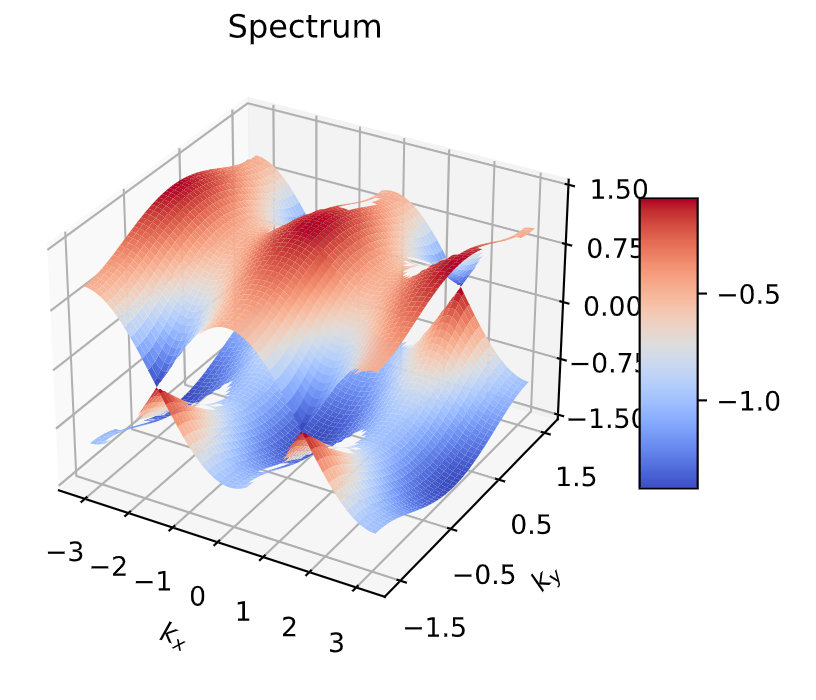
\includegraphics[height=6cm, width=9.5cm]{Spectrum.jpg}
	\caption{Spectrum of the $\pi$-flux model.}
	\end{minipage}
	\hfill
	\begin{minipage}[t]{0.5\linewidth}
	\centering
	\includegraphics[height=6cm,width=8.5cm]{DOS.png}
	\caption{DOS of the 0-flux and $\pi$-flux Hubbard model at different dopping.}
	\end{minipage}
\end{figure}

\section{symmetry analysis}
The symmetry point group of Brillouin zone is $D_{2h} = D_2 \otimes i$, and the character table is shown below
$$
\begin{array}{|l|l|l|l|l|l|l|l|l|l|l|l|}
\hline \mathrm{D}_{2 \mathrm{h}} & \mathrm{E} & \mathrm{C}_{2}(\mathrm{z}) & \mathrm{C}_{2}(\mathrm{y}) & \mathrm{C}_{2}(\mathrm{x}) & \mathrm{i} & \sigma(\mathrm{xy}) & \sigma(\mathrm{xz}) & \sigma(\mathrm{yz}) & \begin{array}{c}
\text { linear} \\
\text{functions}
\end{array} & \begin{array}{l}
\text { quadratic } \\
\text { functions }
\end{array} & \begin{array}{c}
\text { cubic } \\
\text { functions }
\end{array} \\
\hline \mathrm{A}_{\mathrm{g}} & +1 & +1 & +1 & +1 & +1 & +1 & +1 & +1 & - & \mathrm{x}^{2}, \mathrm{y}^{2}, \mathrm{z}^{2} & - \\
\hline \mathrm{B}_{1 \mathrm{g}} & +1 & +1 & -1 & -1 & +1 & +1 & -1 & -1 & \mathrm{R}_{\mathrm{z}} & \mathrm{xy} & - \\
\hline \mathrm{B}_{2 \mathrm{g}} & +1 & -1 & +1 & -1 & +1 & -1 & +1 & -1 & \mathrm{R}_{\mathrm{y}} & \mathrm{xz} & - \\
\hline \mathrm{B}_{3 \mathrm{g}} & +1 & -1 & -1 & +1 & +1 & -1 & -1 & +1 & \mathrm{R}_{\mathrm{x}} & \mathrm{yz} & - \\
\hline \mathrm{A}_{\mathrm{u}} & +1 & +1 & +1 & +1 & -1 & -1 & -1 & -1 & - & - & \mathrm{xyz} \\
\hline \mathrm{B}_{1 \mathrm{u}} & +1 & +1 & -1 & -1 & -1 & -1 & +1 & +1 & \mathrm{z} & - & \mathrm{z}^{3}, \mathrm{y}^{2} \mathrm{z}, \mathrm{x}^{2} \mathrm{z} \\
\hline \mathrm{B}_{2 \mathrm{u}} & +1 & -1 & +1 & -1 & -1 & +1 & -1 & +1 & \mathrm{y} & \mathrm{yz}^{2}, \mathrm{y}^{3}, \mathrm{x}^{2} \mathrm{y} & -  \\
\hline \mathrm{B}_{3 \mathrm{u}} & +1 & -1 & -1 & +1 & -1 & +1 & +1 & -1 & \mathrm{x} & \mathrm{xz}^{2}, \mathrm{xy}^{2}, \mathrm{x}^{3} & - \\
\hline
\end{array}$$
the corresponding wave functions are:
\begin{equation}
	\begin{aligned}
	A_{g} & : \psi  \sim x^2 \text{ or } y^2 \\
	B_{1 g} &: \psi \sim xy \\
	B_{2u} &: \psi \sim y^3 \text{ or } x^2y\\
	B_{3u} &: \psi \sim x^3 \text{ or } xy^2
	\end{aligned}
	\end{equation}
	(with the association $x \rightarrow \sin k_{x}, x^{2} \rightarrow \cos k_{x},$ etc $)$
\section{RG analysis for the Hubbard model on the square lattice}
The standard RG analysis we are going to do is to integrate out the region down to $\Omega_0$. In the particle channel, 2 particle with $\sigma,\sigma^\prime$ and momenta $\vec{k}, -\vec{k}$ interact and 
turn into a pair with the same spin polarization and momenta $\vec{q}, -\vec{q}$. According to the symmetry of the superconductivity, pairs can be classified into singlet and triplet channels, according to their total spin.\par 
The corresponding vertex functions are the 4-point vertex which can be expressed into diagrammatic forms(up to 2PI diagram and $\mathcal{O}(U^4)$):
	\begin{figure}[htbp]
		\begin{minipage}[t]{0.4\linewidth}
		\centering
		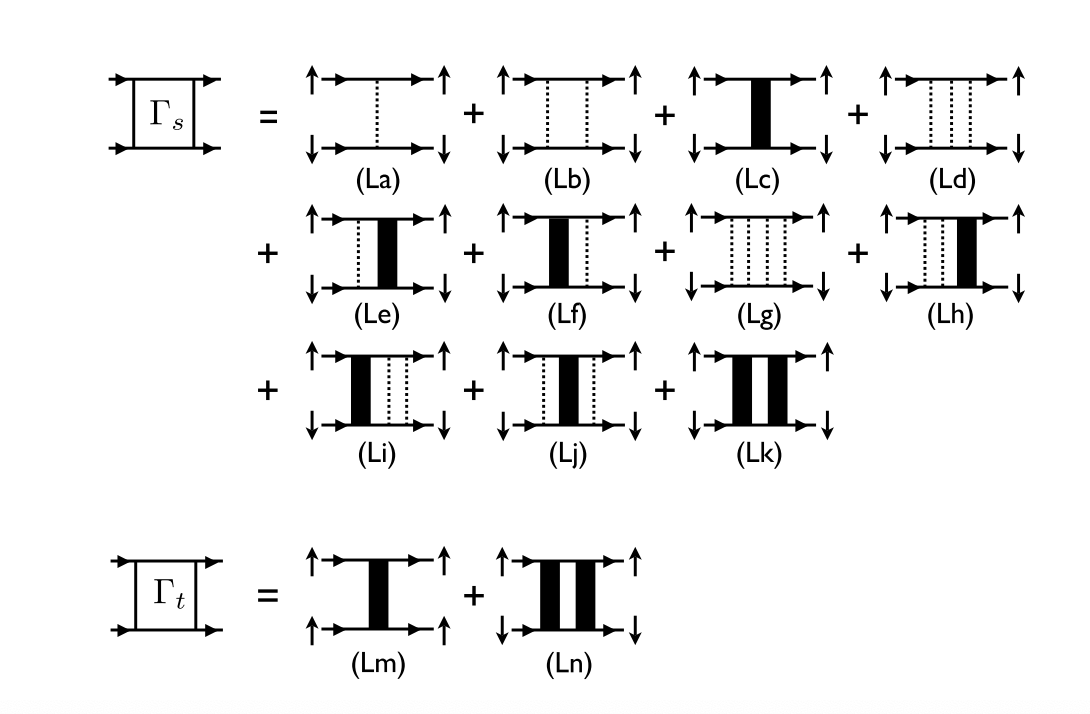
\includegraphics[height=6cm,width=9.5cm]{截屏2020-10-18 下午4.18.55.png}
		\caption{vertex diagrams up to $\mathcal{O}(U^4)$.}
		\end{minipage}
		\hfill
		\begin{minipage}[t]{0.5\linewidth}
		\centering
		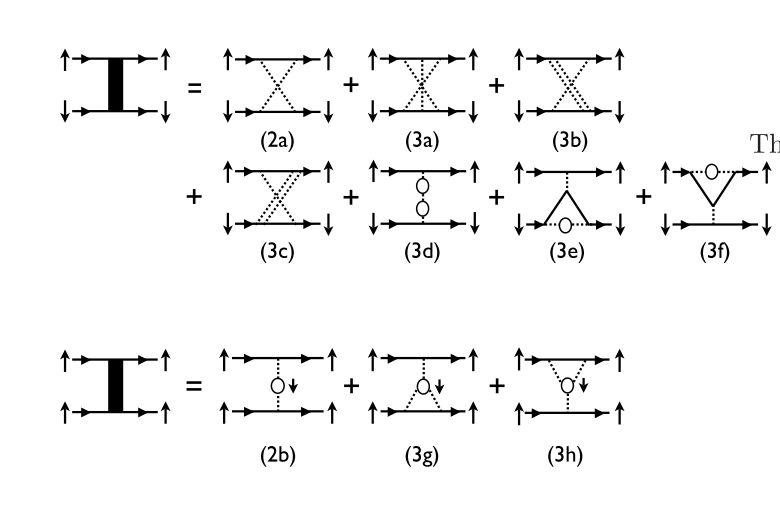
\includegraphics[height=6cm,width=7.5cm]{截屏2020-10-19 上午10.58.17.png}
		\caption{2PI diagrams up to third order.}
		\end{minipage}
	\end{figure}
It is obvious to see that 
\begin{equation}
	\begin{aligned}
\Gamma_{s}\left(\vec{k}, \vec{q} ; \Omega_{0}\right)=U+\sum_{n \geq 2} U^{n} \Gamma_{s}^{(n)}\left(\vec{k}, \vec{q} ; \Omega_{0}\right)
	\end{aligned}
\end{equation}
\begin{equation}
	\Gamma_{t}\left(\vec{k}, \vec{q} ; \Omega_{0}\right)=\sum_{n \geq 2} U^{n} \Gamma_{t}^{(n)}\left(\vec{k}, \vec{q} ; \Omega_{0}\right)
	\end{equation}
\subsection{second order vertex function}
First analyze the singlet vertex function to the second order:
\begin{equation}
	\Gamma_{s}^{(2)}\left(\vec{k}, \vec{q} ; \Omega_{0}\right)=\chi\left(\vec{k}+\vec{q} ; \Omega_{0}\right)+P\left(\Omega_{0}\right)
	\end{equation}
	First we introduce the definition as a notational convenience:
	\begin{equation}
		\sum_{p} =\sum_{\vec{p}}\sum_n \equiv \int_{\Omega_{0}} \frac{d p_{0} d^{d} p}{(2 \pi)^{d+1}}
		\end{equation}
		$p_0$ is the wellknown Matsubara frequency $\omega_m$.(Of course you can write into the form of sum $\sum_{n}$, which is the notation I will take.) The first second order contribution is the polarization operator $\Pi^{0}\left(\mathbf{p}, p_{0}\right)$ we met in RPA and is calculated below in a much more general form:
		\begin{equation}
			\Pi^{0}\left(\mathbf{q}, \omega_{m}\right)\sim \sum_{\vec{k}^{\prime} \sigma^{\prime} n^{\prime}} G^{0}\left(\vec{k}^{\prime} \sigma^{\prime}, \omega_{n^{\prime}}\right) G^{0}\left(\vec{k}^{\prime}+\vec{q} \sigma^{\prime}, \omega_{n^{\prime}}+\omega_{m}\right)
			\end{equation}
Ignoring the sum of spin which only contribute constant multiples and express the free Green function as 
\begin{equation}
	G_0(\vec{k},\omega_n)=\frac{e^{i \omega_{n} 0^{+}}}{i \omega_{n}-\epsilon_{\vec{k}}}
\end{equation}
	So the polarization operator can be further expressed as:
	\begin{equation}
		\begin{aligned}
			\Pi_{0}\left(\vec{q}, \omega_{m}\right)  = &\frac{2}{\beta V} \sum_{\vec{k}} \sum_{n=-\infty}^{\infty} \frac{e^{i \omega_{n} 0^{+}}}{\left(i \omega_{n}-\epsilon_{\vec{k}} \right)\left(i \omega_{n}+i \omega_{m}-\bar{\epsilon}_{\vec{k}+\vec{q}}\right)} \\
			=& \frac{2}{\beta V} \sum_{\vec{k}} \frac{1}{i \omega_{m}-\left(\bar{\epsilon}_{\vec{k}+\vec{q}}-\epsilon_{\vec{k}}\right) } \\
			& \times \sum_{n=-\infty}^{\infty}\left(\frac{e^{i \omega_{n} 0^{+}}}{i \omega_{n}-\epsilon_{\vec{k}} }-\frac{e^{i \omega_{n} 0^{+}}}{i \omega_{n}+i \omega_{m}-\epsilon_{\vec{k}+\vec{q}}}\right)
		\end{aligned}
		\end{equation}
		Using the contour integration we may find the sum of all is
		\begin{equation}
			\sum_{n=-\infty}^{\infty} \frac{e^{i \omega_{n} 0^{+}}}{i \omega_{n}-\epsilon_{\vec{k}} }=\beta f_{\vec{k}}, \sum_{n=-\infty}^{\infty} \frac{e^{i \omega_{n} 0^{+}}}{i \omega_{n}+i \omega_{m}-\epsilon_{\vec{k}+\vec{q}} }=\frac{\beta }{e^{\beta \epsilon_{\vec{k}+\vec{q}}} e^{-i \beta \omega_{m}}+1}=\frac{\beta}{e^{\beta\epsilon_{\vec{k}+\vec{q}}}+1}=\beta f_{\vec{k}+\vec{q}}
		\end{equation} 
The polarization operator of noninteracting electrons is reduced to
\begin{equation}
	\Pi^{0}\left(\vec{q}, \omega_{m}\right)=\frac{2}{V} \sum_{\vec{k}} \frac{f_{\vec{k}}-f_{\vec{k}+\vec{q}}}{i \omega_{m}+\epsilon_{\vec{k}}-\epsilon_{\vec{k}+\vec{q}}}
	\end{equation}
In our case, $\vec{k}$ is set to $\vec{p}$, $\vec{q}$ is set to $-2\vec{p}$. And the general case form of the polarization operator is 
\begin{equation}
	\begin{aligned}
	\Gamma_{s}\left(L_{b}\right) & =\sum_{p} G_{0}(p) G_{0}(-p)\\
		& = \sum_{\vec{p}}\sum_{n=-\infty}^{\infty}\frac{e^{i \omega_{n} 0^{+}}}{\left(i \omega_{n}-\epsilon_{\vec{p}} \right)\left(-i \omega_{n}-\epsilon_{-\vec{p}}\right)}\\
		& =\sum_{\vec{p}}\sum_{n=-\infty}^{\infty}-\frac{1}{2\epsilon_{\vec{p}}}\left(\frac{e^{i\omega 0^+}}{i\omega_n-\epsilon_{\vec{p}}}-\frac{e^{i\omega_n 0^+}}{i\omega_n+\epsilon_{\vec{p}}}\right)\\
		& =\sum_{\vec{p}}-\frac{1}{2\epsilon_{\vec{p}}}(\beta f_{\vec{p}}-\beta f_{-\vec{p}})\\
		& =\sum_{\vec{p}}-\frac{1}{2\epsilon_{\vec{p}}}(\beta f_{\vec{p}}-\beta (1-f_{\vec{k}}))\\
		& = \beta\int_{\Omega_{0}} \frac{d^{d} p}{(2 \pi)^{d}}\left[\frac{1-2 f_{\vec{p}}}{2 \epsilon_{\vec{p}}}\right]
	\end{aligned}
	\end{equation}
We have set the cut off $\Omega_0$, in the case that $d=2$, we have $\int d^2k=2\pi\int_{\Omega_0}kdk$ (in the low temperature limit).
\begin{equation}
	\begin{aligned}
\int_{\Omega_0}dpp\frac{1-2 f_{\vec{p}}}{2 \epsilon_{\vec{p}}}  & = \int_{\Omega_0}dpp\frac{1-2\Theta(\epsilon_{F}-\epsilon_{\vec{p}})}{2\epsilon_{\vec{p}}}\\
& \sim \int dp \Theta(-\vec{p}_{\Omega_0}+\vec{p})\frac{1-2\Theta(\epsilon_{F}-\epsilon_{\vec{p}})}{p}\\
& \sim \rho\log[A/\Omega_0]
	\end{aligned}
\end{equation}\footnote{How to determine the parameter A? I can only derive the logarithmic divergence. The intergration is a difficulty for me.}
Meanwhile, the diagram in 2PI labeled by $U^2$ is regular. 
\begin{equation}
	\begin{aligned}
	\Sigma^{(2)}\left(\vec{k} ; \Omega_{0}\right) &=\int_{\Omega_{0}} \frac{d \vec{q} d \omega}{(2 \pi)^{d+1}} G(\vec{k}+\vec{q}, \omega) G(\vec{q}, \omega) \\
	& \equiv \chi\left(\vec{k} ; \Omega_{0}\right)
	\end{aligned}
	\end{equation}
\begin{equation}
	\begin{aligned}
	\sum_{p}G(\vec{k}+\vec{q},\omega)G(\vec{q},\omega) & =\sum_{\vec{p}}\sum_{n=-\infty}^{\infty}\frac{e^{i \omega_{n} 0^{+}}}{\left(i \omega_{n}-\epsilon_{\vec{k}+\vec{q}} \right)\left(i \omega_{n}-\epsilon_{\vec{q}}\right)}\\
	& =\sum_{\vec{p}}\sum_{n=-\infty}^{\infty}\frac{1}{\epsilon_{\vec{q}}-\epsilon_{\vec{k}+\vec{q}}}\left(\frac{e^{i\omega_n0^+}}{i\omega_n-\epsilon_{\vec{k}+\vec{q}}}-\frac{e^{i\omega_n0^+}}{i\omega_n-\epsilon_{\vec{q}}}\right)\\
	& =\sum_{\vec{p}}\frac{f_{\vec{k}+\vec{q}}-f_{\vec{q}}}{\epsilon_{\vec{q}}-\epsilon_{\vec{k}+\vec{q}}}
	\end{aligned}
\end{equation}
\begin{equation}
	\Gamma_{s}(2 a)=\sum_{p} G_{0}(p) G_{0}(k+q+p)=\chi(\vec{k}+\vec{q})+\mathcal{O}\left(\Omega_{0}\right)
	\end{equation}
As we can see from the diagram(2a) that the particle-hole bubble $\chi$ is regular while the particle-particle bubble has the logarithmic divergence. 
So the singlet vertex function up to second order is 
\begin{equation}
	\Gamma_{s}\left(\vec{k}, \vec{q} ; \Omega_{0}\right)=U+ U^2(\chi(\vec{k}+\vec{q} ; \Omega_{0})+P\left(\Omega_{0}\right))
	\end{equation}
By the same analysis, we find the triplet vertex function up to second order is 
\begin{equation}
	\Gamma_{t}\left(\vec{k}, \vec{q} ; \Omega_{0}\right)=-U^2\chi(\vec{k}-\vec{q};\Omega_0)
	\end{equation}
\subsection{higer order vertex function}
	For the higher order vertex, there are some terms that differ from all in the second order vertex function. Since we only care about the divergence, a so-call "asymptotically" analysis can be applied.
	For example the diagram in ($L_d$) contribute the main divergence
	\begin{equation}
		\Gamma_{s}\left(L_{d}\right)=\left[\sum_{p} G_{0}(p) G_{0}(-p)\right]^{2}=\rho^{2} \log ^{2}\left[A / \Omega_{0}\right]
		\end{equation}
The second important contribution of the diagrams comes from ($L_c$) and ($L_f$),
\begin{equation}
	\begin{aligned}
	\Gamma_{s}^{(3)}\left(L_{e}\right)=& \sum_{p p^{\prime}} G_{0}\left(q+p+p^{\prime}\right) G_{0}\left(p^{\prime}\right) G_{0}(p) G_{0}(-p) \\
	=&\left[\sum_{p} \chi(\vec{q}+\vec{p})\left[G_{0}(p) G_{0}(-p)\right]+\mathcal{O}\left(\Omega_{0}\right)\right]+\delta \Gamma_{s}\left(L_{e}\right)
	\end{aligned}
	\end{equation}
where
\begin{equation}
	\delta \Gamma_{s}\left(L_{e}\right)=\sum_{p}\left[\chi\left(\vec{q}+\vec{p} ; i p_{0}\right)-\chi(\vec{q}+\vec{p}, 0)\right] G_{0}(p) G_{0}(-p)
	\end{equation}
It is obivious to prove this, when we express the Green function into sum of Matsubara frequency:
\begin{equation}
	\begin{aligned}
\sum_{pp^\prime}G_0(q+p+p^\prime)G_0(p^\prime)G_0(p)G_0(-p) & = \sum_{p}\sum_{\vec{p^\prime}}\sum_{n=-\infty}^{\infty}\frac{e^{i \omega_{n} 0^{+}}}{\left(i \omega_{n}-\epsilon_{\vec{q}+\vec{p}+\vec{p^\prime}} \right)\left(i \omega_{n}+i\omega_{m}-\epsilon_{\vec{p^\prime}}\right)}G_0(p)G_0(-p)\\
& =\sum_{p}\sum_{\vec{p}^\prime}\frac{1}{i\omega_{m}-(\epsilon_{\vec{p^\prime}}-\epsilon_{\vec{q}+\vec{p}+\vec{p}^\prime})}(f_{\vec{q}+\vec{p}+\vec{p}^\prime}-f_{\vec{p}^\prime})G_0(p)G_0(-p)\\
& =\sum_{p}\sum_{\vec{p}^\prime}\frac{1}{i\omega_{m}-(\epsilon_{\vec{p^\prime}}-\epsilon_{\vec{q}+\vec{p}+\vec{p}^\prime})}(f_{\vec{q}+\vec{p}+\vec{p}^\prime}-f_{\vec{p}^\prime})G_0(p)G_0(-p)\\
& +\sum_{p}\sum_{\vec{p}^\prime}\frac{1}{(\epsilon_{\vec{p^\prime}}-\epsilon_{\vec{q}+\vec{p}+\vec{p}^\prime})}(f_{\vec{q}+\vec{p}+\vec{p}^\prime}-f_{\vec{p}^\prime})G_0(p)G_0(-p)\\
& -\sum_{p}\sum_{\vec{p}^\prime}\frac{1}{(\epsilon_{\vec{p^\prime}}-\epsilon_{\vec{q}+\vec{p}+\vec{p}^\prime})}(f_{\vec{q}+\vec{p}+\vec{p}^\prime}-f_{\vec{p}^\prime})G_0(p)G_0(-p)\\
& =\sum_{p}\chi(\vec{k}+\vec{q})[G_0(p)G_0(-p)+\mathcal{O}(\Omega_0)\\
& +\sum_{p}[\chi(\vec{q}+\vec{p},i\omega_n)-\chi(\vec{q}+\vec{p},0)]G_0(p)G_0(-p)
	\end{aligned}
\end{equation}
Where we label the last term by $\delta\Gamma(L_e)$,\footnote{I have not examined whether the term is singular.}
Using the identity
\begin{equation}
	\int_{\Omega_{0}} \frac{d^{d} p}{(2 \pi)^{d}}=\int \frac{d \hat{p}}{S_{F}} \frac{\bar{v}_{F}}{v_{F}(\hat{p})} \int_{|\epsilon|>\Omega_{0}} d \epsilon \rho(\epsilon)
	\end{equation}
	where $\int d\hat{p}$ denotes the integration over the area of the Fermi surface. And we set 
\begin{equation}
		\gamma^{(3)}(\vec{k}) \equiv \int \frac{d \hat{p}}{S_{F}}\left(\frac{\bar{v}_{F}}{v_{F}(\hat{p})}\right) \chi(\vec{k}+\hat{p})
		\end{equation}
So (3.20) can be reduced to 
\begin{equation}
	\begin{aligned}
		 \Gamma_s^{(3)}(L_e)  = & \sum_{p}\chi(\vec{p}+\vec{q})[G_0(p)G_0(-p)+\mathcal{O}(\Omega_0) +\sum_{p}[\chi(\vec{q}+\vec{p},i\omega_n)-\chi(\vec{q}+\vec{p},0)]G_0(p)G_0(-p)\\
		= &\sum_{\vec{p}}\sum_{n=-\infty}^{\infty}\chi(\vec{p}+\vec{q})[G_0(p)G_0(-p)]+\delta\Gamma(L_e)\\
		= &\int_{\Omega_0}\frac{d^dp}{(2\pi)^d}\left(\chi(\vec{p}+\vec{q})\frac{1-2f(\epsilon_{\vec{p}})}{2\epsilon_{\vec{p}}}\right)+\delta\Gamma(L_e)\\
		= &\int \frac{d \hat{p}}{S_{F}} \frac{\bar{v}_{F}}{v_{F}(\hat{p})} \chi(\hat{p}+\vec{q})\int_{|\epsilon|>\Omega_{0}} d \epsilon \rho(\epsilon)\frac{1-2f_{\vec{p}}}{2\epsilon_{\vec{p}}}+\delta\Gamma(L_e)\\
		= & \gamma^{(3)}(\vec{q})\rho\log[A/\Omega_0]+\delta\Gamma(L_e)
	\end{aligned}
\end{equation}
Which is the same as $(L_f)$. The remaining terms in the diagrams are non-singular and can be easily read from 2PI diagram.
\begin{equation}
	\begin{aligned}
	\Gamma_{s}(3 a) &=\sum_{p p^{\prime}} G_{0}(p) G_{0}(k+q+p) G_{0}\left(p^{\prime}\right) G_{0}\left(k+q+p^{\prime}\right) 
	=\chi^{2}(\vec{k}+\vec{q})+\mathcal{O}\left(\Omega_{0}\right)
	\end{aligned}
	\end{equation}
	\begin{equation}
		\Gamma_{s}(3 b)=\Gamma_{s}(3 c)=\sum_{p p^{\prime}} G_{0}(p) G_{0}\left(q+p^{\prime}-p\right) G_{0}\left(p^{\prime}\right) G_{0}\left(k+q+p^{\prime}\right)
		\end{equation}
		\begin{equation}
			\Gamma_{s}(3 d)=\chi^{2}(\vec{k}-\vec{q})
			\end{equation}
			\begin{equation}
				\Gamma_{s}(3 e)=-\sum_{p p^{\prime}} G_{0}(p) G_{0}(p+k-q) G_{0}\left(p^{\prime}\right) G_{0}\left(p^{\prime}-k-p\right)
				\end{equation}
Thus, split the singular part and the non-singular part, the vertex function up to 3 order can be expressed as
\begin{equation}
	\Gamma_{s}^{(3)}\left(\vec{k}, \vec{q} ; \Omega_{0}\right)=\rho^{2} \log ^{2}\left[A / \Omega_{0}\right]+\left[\gamma^{(3)}(\vec{k})+\gamma^{(3)}(\vec{q})\right] \rho \log \left[A / \Omega_{0}\right]+\tilde{\Gamma}_{s}^{(3)}(\vec{k}, \vec{q})+\mathcal{O}\left(\Omega_{0}\right)
	\end{equation}
Where the $\tilde{\Gamma}_{s}^{(3)}(\vec{k}, \vec{q})$ is the non-singular part.\par 
The same treatment to the triplet.
The lowest order contribution comes from $(2b)$
	\begin{equation}
	  \Gamma_{t}(2b)=-\chi(\vec{k}-\vec{q})+\mathcal{O}(\Omega_0)
		\end{equation}
The third order comes from the $(L_m)$
			\begin{equation}
				\begin{aligned}
				\Gamma_{t}(3 g) &=-\sum_{p p^{\prime}} G_{0}(p) G_{0}(k-q+p) G_{0}\left(p^{\prime}\right) G_{0}\left(k+p+p^{\prime}\right) \\
				&=-\sum_{p} G_{0}(p) G_{0}(k-q+p) \chi(k+p)+\mathcal{O}(\Omega_0)
				\end{aligned}
				\end{equation}
The divergence occurs at the fourth order, which has the form of
\begin{equation}
	\Gamma_{t}\left(L_{n}\right)=\rho \log \left[A / \Omega_{0}\right] \gamma_{t}^{(4)}(\vec{k}, \vec{q})+\mathcal{O}\left(\Omega_{0}\right)
	\end{equation}
where
\begin{equation}
	\gamma_{t}^{(4)}(\vec{k}, \vec{q})=\int \frac{d \hat{p}}{S_{F}} \chi(\vec{k}-\hat{p})\left(\frac{\bar{v}_{F}}{v_{F}(\hat{p})}\right) \chi(\vec{p}-\hat{q})
	\end{equation}
\section{RG analysis II:}
The remaining states lie in a narrow strip of width $\Omega_0$ about the Fermi surface so that the spectrum can be linearized without loss of accuracy.
The only couplings that renormalize are those in the Cooper channel.\par 
The form of the vertex function can be treated as a matrix labeled by $\vec{k},\vec{q}$, we define a quantity
\begin{equation}
	g_{\hat{k}, \hat{q}} \equiv \rho \sqrt{\frac{\bar{v}_{F}}{v_{F}(\hat{k})}} \Gamma(\hat{k}, \hat{q}) \sqrt{\frac{\bar{v}_{F}}{v_{F}(\hat{q})}}
	\end{equation}
It is easy to examine $g_{\vec{k,\vec{q}}}$ is a symmetric and real matrix. Diagonalize the matrix to make the eigenvalues decoupled. 
\begin{equation}
	g_{\hat{k}, \hat{q}}^{0}=\sum_{n} \lambda_{n}^{0} \psi_{n}^{\star}(\hat{k}) \psi_{n}(\hat{q})
	\end{equation}
Each eigenvalue renormalizes independently:
\begin{equation}
	\frac{d \lambda_{n}}{d \ell}=-\lambda_{n}^{2} ; \quad \lambda_{n}(\Omega)=\frac{\lambda_{n}^{0}}{1+\lambda_{n}^{0} \log \left[\Omega_{0} / \Omega\right]}
	\end{equation}
Among all the possible solutions, we identify the most negative eigenvalue $\lambda_0$, then
\begin{equation}
	T_c\sim \mu \exp[-1/|\lambda_0|]
\end{equation}
\section{Numerical study}
To discretize the Fermi surface, we have to decide the pattern of them, set the Fermi energy to 0, and we are able to draw Fermi surface at different dopping.\par 

Focusing on the band above we find that there are 4 fermi pockets at low doping as the blue and the red contour line show. At the electron concentration of  $n\approx 0.29285$, the topology of the fermi surface changes
as shown in the black dashed contour line. When the electron concentration is higher than 0.29285, the 3 hole pockets turn into 3 Fermion pockets as shown in the dashed contour line. The change of the topology indicates the Van Hove Singularity, as is shown in the Figure2, reminds us to discretize the 
Fermi surface with caution. There are 4 Van Hove singularities in 1BZ.\par 

\begin{figure}[htbp]
	\begin{minipage}[t]{0.5\linewidth}
	\centering
	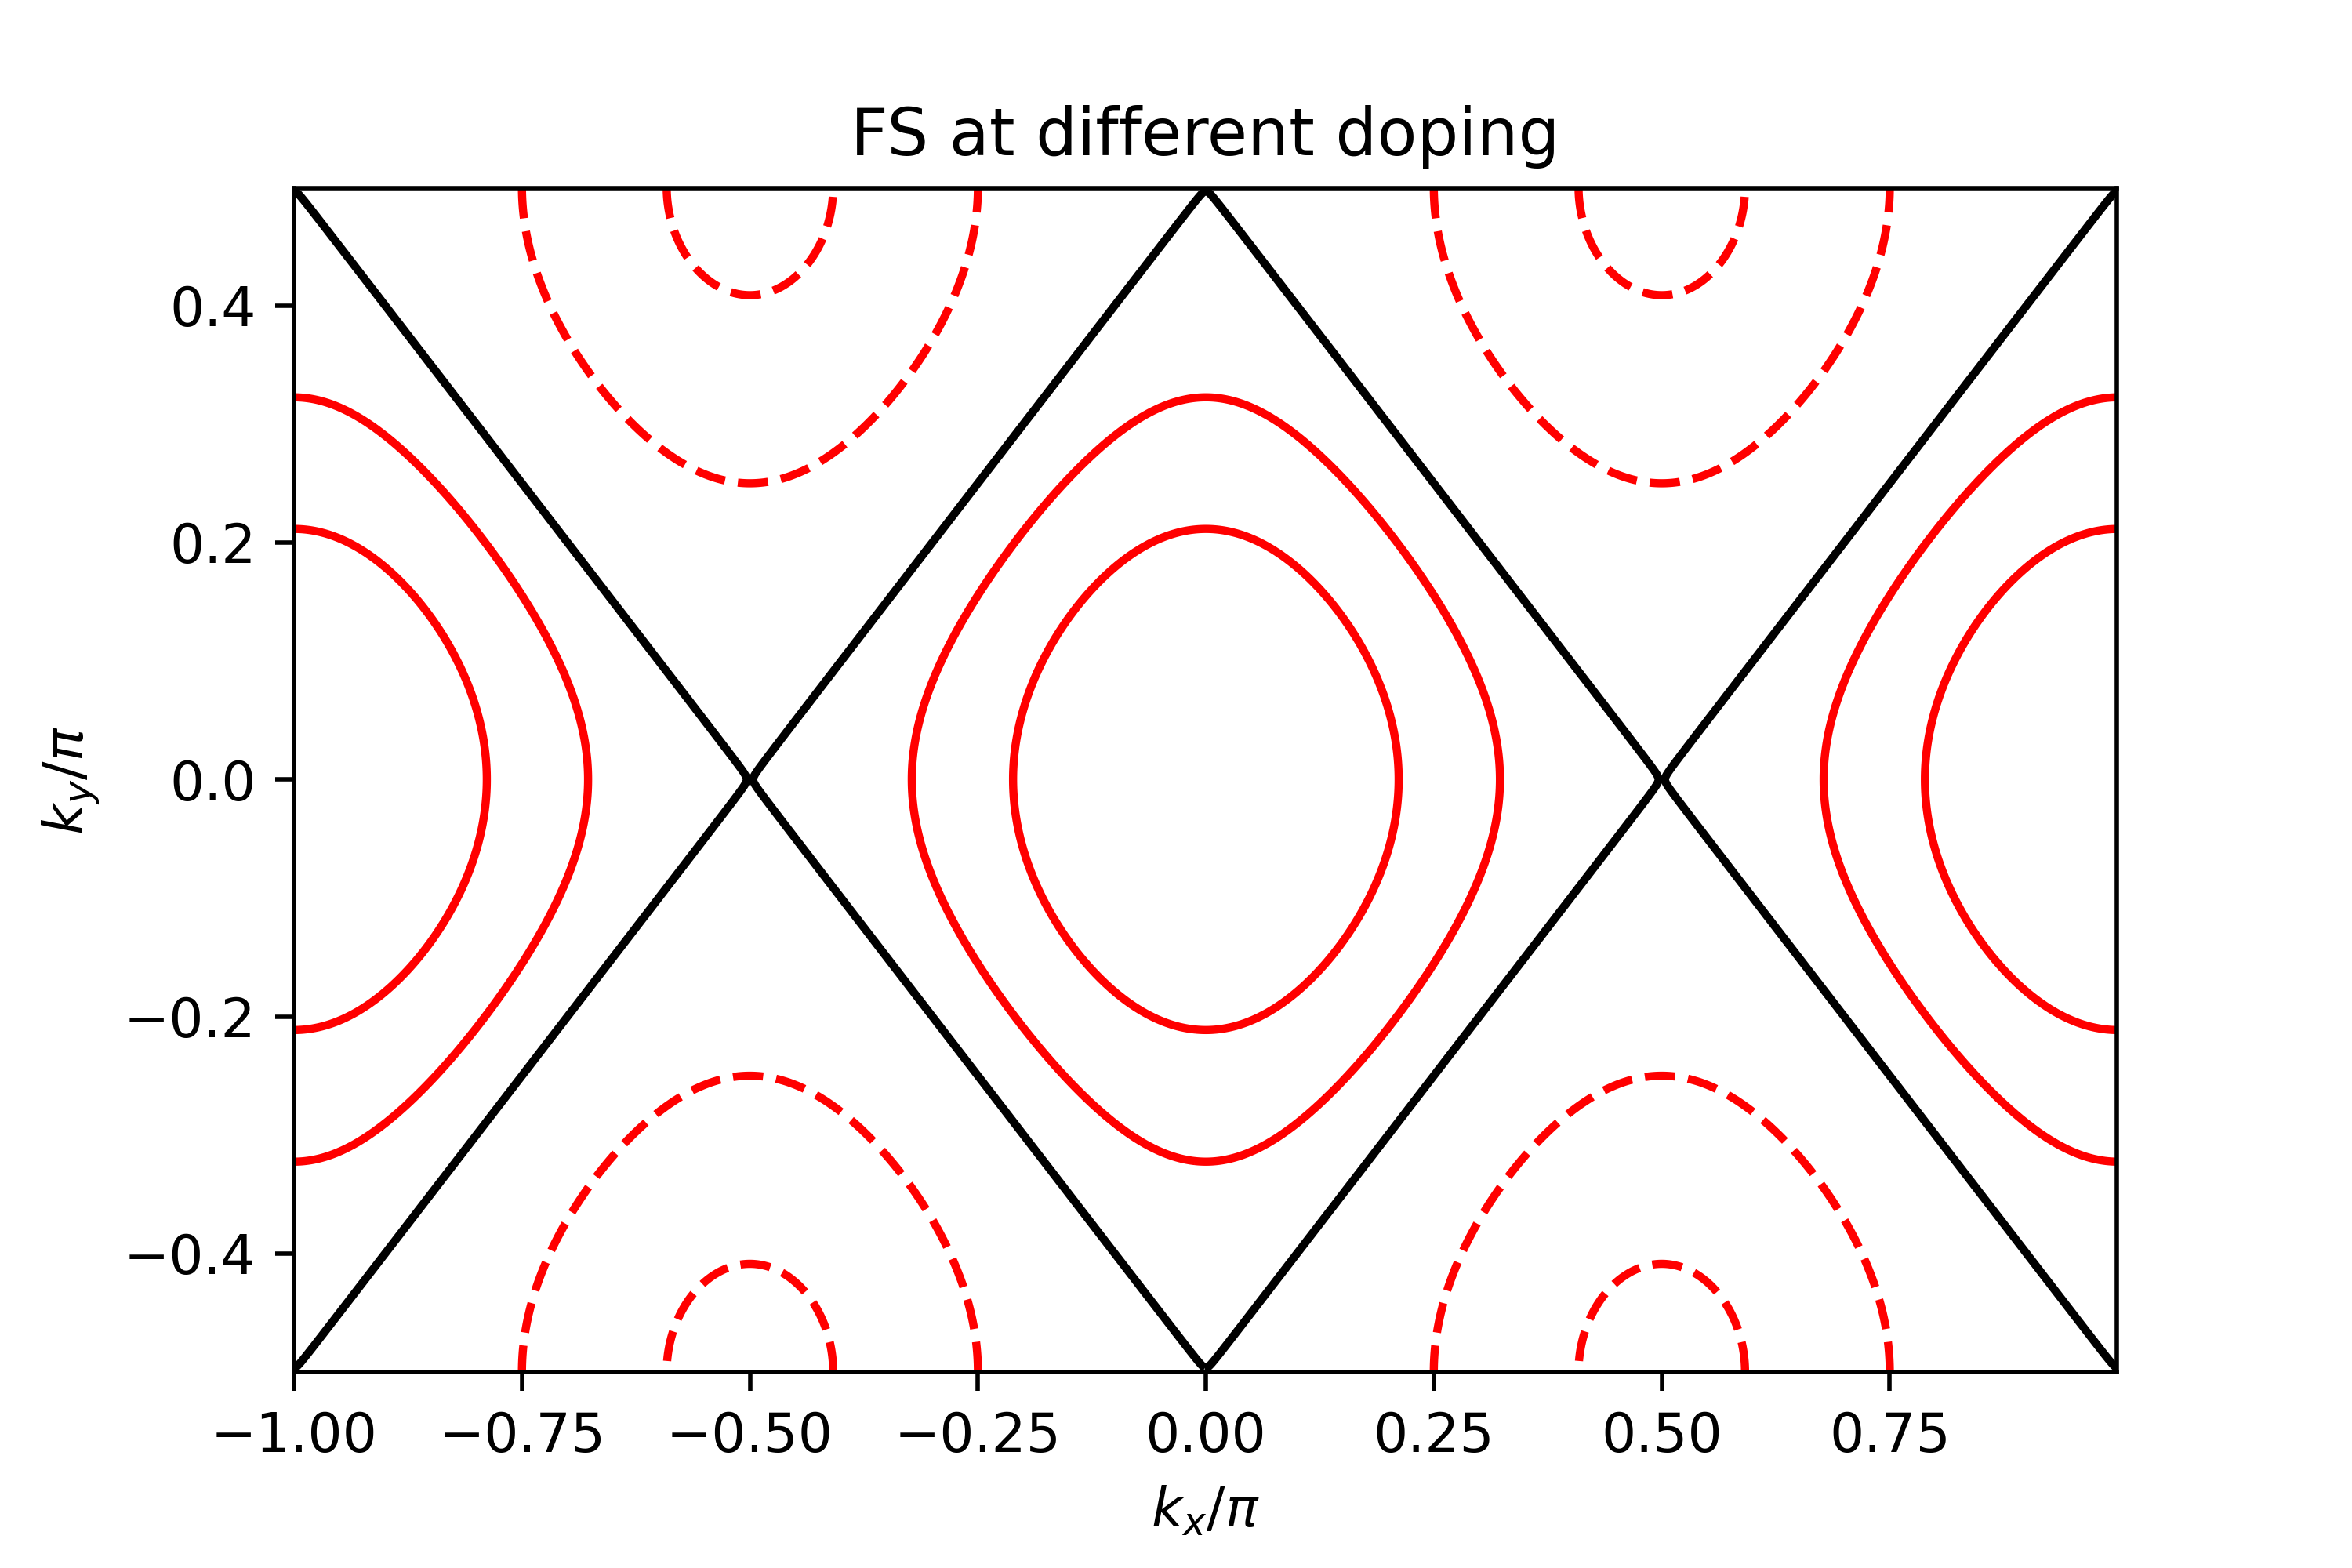
\includegraphics[height=6cm,width=9.5cm]{Fermisurface.png}
	\caption{Fermi surface at different doping. The dashed red contour is the hole pockets while the solid red line contour is the Fermion pockets. The black solid line indicates the Van Hove singularity.}
	\end{minipage}
	\hfill
	\begin{minipage}[t]{0.5\linewidth}
	\centering
	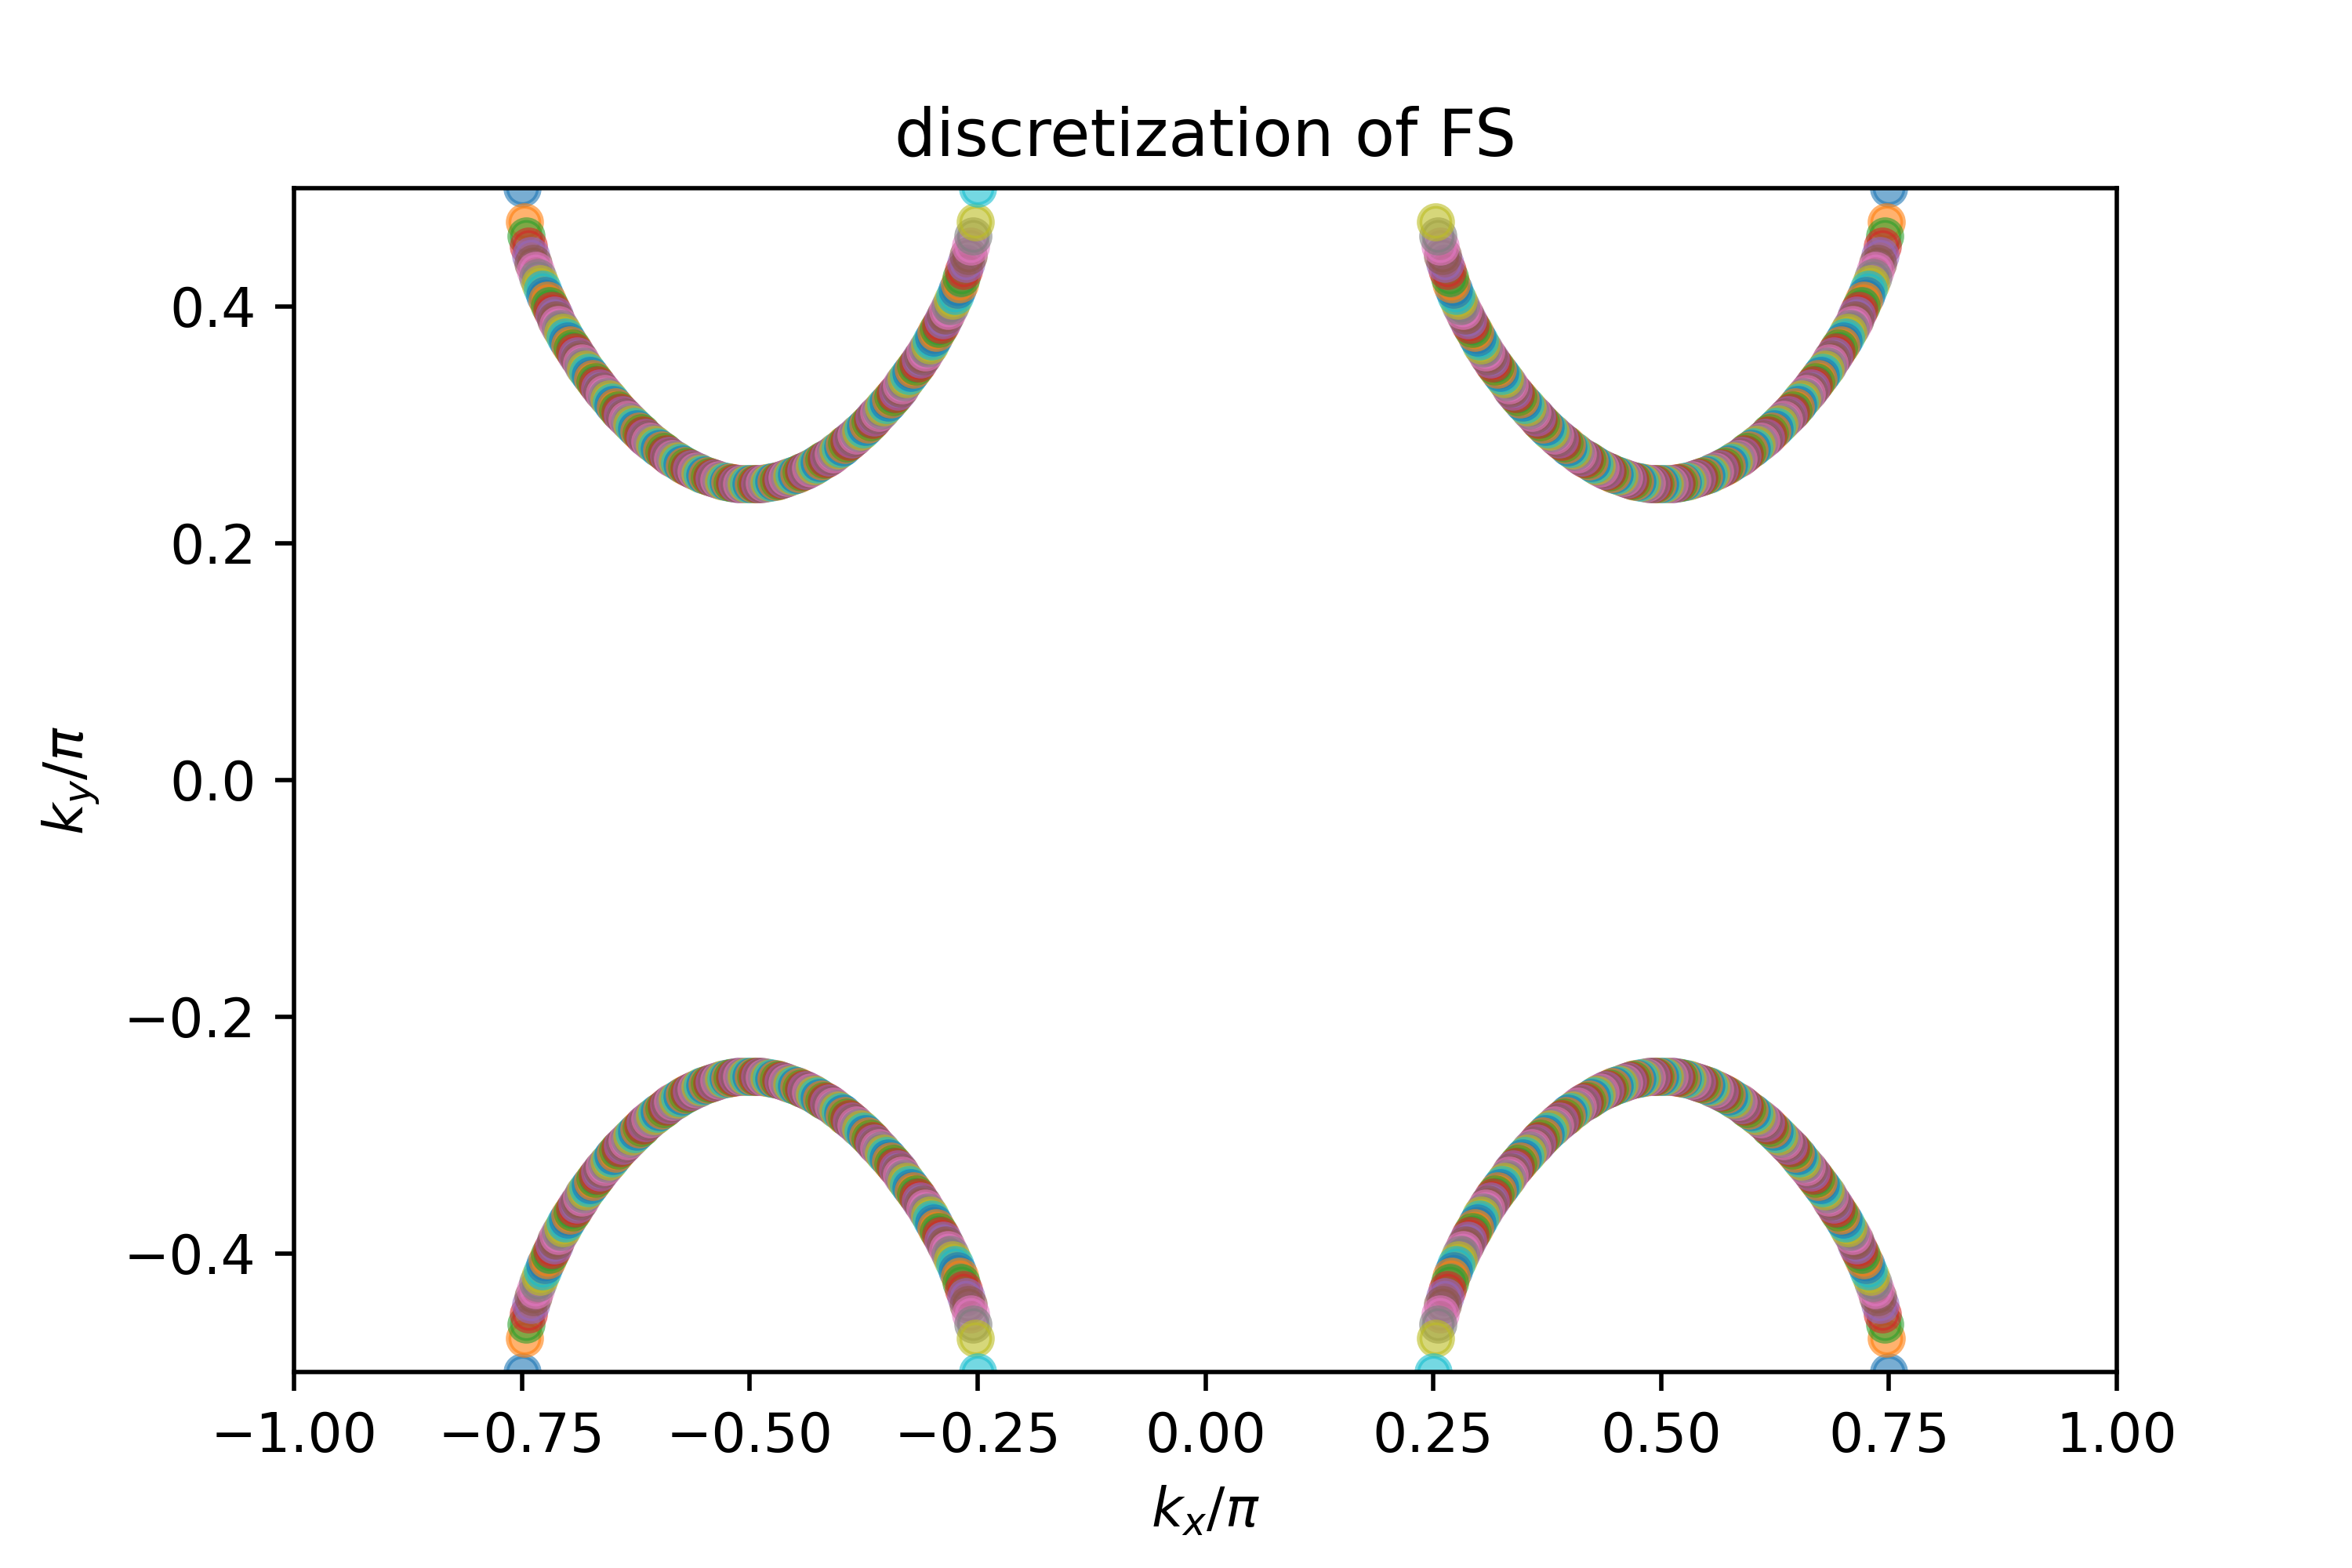
\includegraphics[height=6cm,width=9.5cm]{DFS.png}
	\caption{discretization of FS.(n=0.2)}
	\end{minipage}
\end{figure}
After the discretization of Fermi/hole pockets, we may calculate the relevant function to consruct the $\Gamma$ matrix. Most of the functions can be directly calculated, including the magnetic susceptibility in zero temperature limit.
\begin{equation}
	\begin{aligned}
	\chi(\vec{k}) & = -\int \frac{d^2q}{(2\pi)^2} \frac{f_{\vec{k}+\vec{q}}-f_{\vec{q}}}{\epsilon_{\vec{k+q}}-\epsilon_{\vec{q}}}\\
	\end{aligned}
\end{equation} 
for the $\epsilon_{\vec{k}+\vec{q}}, \epsilon_{\vec{q}}<<k_BT$, we may replace the $f_{\vec{k}+\vec{q}}$ into step function, the constraint of the step function limits the intergration area. Thus we translate the magnetic susceptibility into the form for numerical study. 
\begin{equation}
	\begin{aligned}
	\chi(\vec{k}) = \int_{FS} \frac{d^2q}{(2\pi)^2} \frac{\Theta(\epsilon_{\vec{k}+\vec{q}}-\epsilon_F)-\Theta(\epsilon_{\vec{q}}-\epsilon_F)}{\epsilon_{\vec{k}+\vec{q}}-\epsilon_{\vec{q}}}\\
	\end{aligned}
\end{equation} 

\section{Mean Field Treatment}
\subsection{BCS state}
Meanfield treatment is the fundamental methods of the BCS theory. Consider the BCS interaction:
\begin{equation}
	H_{B C S}=-\frac{U}{V} \sum_{\vec{k} \vec{k}^{\prime} \tau} c_{\vec{k} \uparrow\tau }^{\dagger} c_{-\vec{k} \downarrow\tau }^{\dagger} c_{-\vec{k}^{\prime} \downarrow \tau} c_{\vec{k}^{\prime} \uparrow \tau}\quad \tau = A,B
	\end{equation}

Ignore the flucuation and substitute the corresponding operator into average value, rewrite the Hamiltonian into Bdg form. We compose the interaction into the product of the form factor and preserve the maximum $\lambda_i$ as $\lambda$.
\begin{equation}
	U =\sum_{i}\lambda_i f^i_{\vec{k}} f^{i*}_{\vec{k}^\prime}
\end{equation}
define
\begin{equation}
	\Delta=\frac{\lambda}{V} \sum_{\vec{k}} f_{\vec{k}}^{*}\left\langle c_{\vec{k}}^{\dagger} c_{-\vec{k}}^{\dagger}\right\rangle=\frac{\lambda}{V} \sum_{\vec{k}} f_{\vec{k}}\left\langle c_{-\vec{k}} c_{\vec{k}}\right\rangle
	\end{equation}
Choose \begin{equation}
	\psi_{\vec{k}}=\left(c_{A, \vec{k} \uparrow}, c_{B, \vec{k} \uparrow}, c_{A,-\vec{k} \downarrow}^{\dagger}, c_{B,-\vec{k} \downarrow}^{\dagger}\right)^{T}
	\end{equation}
as Nambu Spinor, the standard BdG form of the Hamiltonian is 
\begin{equation}
	\left(\begin{array}{cccc}
		c_{A, \vec{k} \uparrow}^\dagger, c_{B, \vec{k} \uparrow}^\dagger, c_{A,-\vec{k} \downarrow}, c_{B,-\vec{k} \downarrow}
	\end{array}\right) \underbrace{\left(\begin{array}{cccc}
	-2t\cos k_x-\mu & 2t\cos k_y & f_{\vec{k}}\Delta & 0 \\
	2t\cos k_y & 2t\cos k_x-\mu & 0 & f_{\vec{k}}\Delta \\
	f_{\vec{k}}\Delta & 0 & 2t\cos k_x-\mu & -2t\cos k_y \\
	0 & f_{\vec{k}}\Delta & -2t\cos k_y & -2t\cos k_x-\mu
	\end{array}\right)}_{\mathcal{H}}\left(\begin{array}{c}
		c_{A, \vec{k} \uparrow}\\
		c_{B, \vec{k} \uparrow}\\
		c_{A,-\vec{k} \downarrow}^{\dagger} \\
		c_{B,-\vec{k} \downarrow}^{\dagger}
	\end{array}\right)
	\end{equation}

	where 
\begin{equation}
	E(\vec{k})=\sqrt{\cos^2 k_x+\cos^2 k_y+\left|f_{\vec{k}}\right|^{2} \Delta^{2}}
	\end{equation}
is the quasiparticle spectrum, and the pairing amplitude ∆ satisfies the standard BCS equation
\begin{equation}
	1=\frac{U}{2 V} \sum_{\vec{k}} \frac{\left|f_{\vec{k}}\right|^{2}}{E(\vec{k})}
	\end{equation}
\subsection{FFLO state}
\begin{equation}
	H_{F F L O}=-\frac{U}{V} \sum_{\vec{k} \vec{k}^{\prime} \tau} c_{\vec{k} \uparrow \tau}^{\dagger} c_{\vec{2Q}-\vec{k} \downarrow \tau}^{\dagger} c_{\vec{k}^{\prime} \downarrow \tau} c_{2\vec{Q}-\vec{k}^{\prime} \uparrow \tau} \quad \tau =A,B
	\end{equation}
	Choose \begin{equation}
		\psi_{\vec{k}}=\left(c_{A, \vec{k} \uparrow}, c_{B, \vec{k} \uparrow}, c_{A,2\vec{Q}-\vec{k} \downarrow}^{\dagger}, c_{B,2\vec{Q}-\vec{k} \downarrow}^{\dagger}\right)^{T}
		\end{equation}
	as Nambu Spinor, the standard BdG form of the Hamiltonian is 
	\begin{equation}
	\left(\begin{array}{cccc}
			c_{A, \vec{k} \uparrow}^\dagger, c_{B, \vec{k} \uparrow}^\dagger, c_{A2\vec{Q}-\vec{k} \downarrow}, c_{B,2\vec{Q}-\vec{k} \downarrow}
		\end{array}\right) \underbrace{\left(\begin{array}{cccc}
		-2t\cos k_x-\mu & 2t\cos k_y & f_{\vec{k}}\Delta & 0 \\
		2t\cos k_y & 2t\cos k_x-\mu & 0 & f_{\vec{k}}\Delta \\
		f_{\vec{k}}\Delta & 0 & 2t\cos (2q_x-k_x)-\mu & -2t\cos (2q_y-k_y) \\
		0 & f_{\vec{k}}\Delta & -2t\cos (2q_y-k_y) & -2t\cos (2q_x-k_x)-\mu
		\end{array}\right)}_{\mathcal{H}}\left(\begin{array}{c}
			c_{A, \vec{k} \uparrow}\\
			c_{B, \vec{k} \uparrow}\\
			c_{A,2\vec{Q}-\vec{k} \downarrow}^{\dagger} \\
			c_{B,2\vec{Q}-\vec{k} \downarrow}^{\dagger}
		\end{array}\right)
	\end{equation}
when $\vec{Q}$ is of poor symmetry, the spectrum can not be solved exactly. However, if we restrict $\vec{Q}$ to $(\pm\frac{\pi}{2},\pm\frac{\pi}{2})$, the quasiparticle spectrum can be calculated directly.
However in our model, the point $2\vec{Q}-\vec{k}$ is out of the 1BZ, which can be modified by shifting a $(0,\pm\pi)$. The operation is equivalent to the FFLO state to $(\pm\frac{\pi}{2},0)$ thus the Hamiltonian turns to
\begin{equation}
\left(\begin{array}{cccc}
	-2t\cos k_x-\mu & 2t\cos k_y & f^*_{\vec{k}}\Delta & 0 \\
	2t\cos k_y & 2t\cos k_x-\mu & 0 & f^*_{\vec{k}}\Delta \\
	f_{\vec{k}}\Delta & 0 & 2t\cos (\pi-k_x)-\mu & -2t\cos (-k_y) \\
	0 & f_{\vec{k}}\Delta & -2t\cos (-k_y) & -2t\cos (\pi-k_x)-\mu
	\end{array}\right)
\end{equation}
the quasiparticle spectrum is 
\begin{equation}
	\begin{aligned}
	E(\vec{k}) & = \sqrt{\cos^2 k_x+\cos^2 k_y+|f_{\vec{k}}|^2\Delta^2+2|f_{\vec{k}}|\Delta\cos k_x }\\ 
& = \sqrt{\cos k_y^2+(\cos k_x +|f_{\vec{k}}|\Delta)^2 }
	\end{aligned}
\end{equation}

\end{document}
